\chapter{Available Frameworks and Related Work}
\label{chap3}

There have already been made significant studies around the subject pf IoT platforms in general and, more specifically, IoT-based solutions for air quality applications too. Projects like SEMAR \cite{SEMARIoTServer}, which is similar to the SYNAISTHISI platform, aim to develop and maintain their implementations based on IoT principles. Additionally, they provide an interface capable of hosting multiple IoT applications. Papers, such as the one in \cite{SEMARkafka}, aim to extend the SEMAR platform with similar implementations, focusing on developing an air pollution monitoring application that leverages real-time air quality detection and integrates tools from the Kafka ecosystem.
Similarly, in paper \cite{HandlingStreamAirPollutionData}, there is an effort to develop a similar application using various tools developed by Apache and other infrastructures focused on IoT. Our objective differentiates us from these efforts, by aiming to develop a platform that not only accommodates to our air quality requirements by supplying all essential components for an air quality application, but also ensures our platform remains scalable, upgradable and highly available across different hosting environments. We leverage technologies, services, methodologies and configurations originating from the enterprise development business (e.g. data validation, fault tolerance, high throughput) and incorporate them into our IoT and open-source based application.

Progressing, another instance is the development of an air pollution monitoring system with sensors on city buses \cite{sensorsoncitybus}. Another one MoreAir \cite{Low-CostUrbanAir} presents an agile and low-cost urban air pollution monitoring system. These provide some comprehensive solutions and implementations of the innovative idea of installing sensors on city buses to gain a more detailed and focusing on low and accessible cost of such infrastructures. While acknowledging the potential of such efforts, some studies analyze the challenges that they have faced \cite{Howfarhavetheygone}, such as the lack of universal applicability of these implementations for specific purposes. Therefore, a significant part of our focus is on the creation and expansion of an upgradable and expandable platform, able to host IoT based applications similar to air quality monitoring. In this regard, we have avoided developing an overly specialized implementation exclusively for our air quality application. Apart from merely implementing and completing the monitoring task, we also emphasize on the services and tools we are integrating into our platform. We develop and optimize our infrastructure for environmental monitoring, showcasing the re-usability of individual services of our stack across similar infrastructures. We aim to categorize our stack in a way that allows groups and layers of our system to be efficiently maintained and upgraded (cf. Sec. \hyperref[system_overview]{4.1}). Lastly, compared to \cite{SEMARkafka} and \cite{HandlingStreamAirPollutionData}, we place a high priority on implementing and developing services maintained by their contributors and the open-source community. This approach ensures our platform remains future-proof and up-to-date with emerging technologies.

\section{Docker}

The primary development environment utilized in this thesis is Docker~\cite{Docker}. All applications are executed in a containerized environment using the Docker engine, a tool renowned in both the IoT and enterprise markets for its efficiency and reliability. Docker is a platform as a service product that provides the ability for services to run on an operating system level virtualization, as shown in Figure \ref{ComparingContainersandVirtualMachines}. Unlike traditional virtual machines, containerized services such as Docker provide enhanced resource efficiency and uniformity across various environments, making them an optimal choice for modern software development due to their reduced system demands and consistent performance. 

Alternative solutions to Docker are Podman, Containerd and LXC (Linux Containers), all of which offer container runtime services. However, Docker stands out due to its simplicity and large user community, that makes it a more accessible and user-friendly option for developers. By adopting this approach, each individual service is isolated from the others , creating a conducive development environment. This allows developers to focus on their workflow for individual services without the concern of compatibility issues, thereby enhancing productivity and efficiency.

\begin{figure}[htbp]
	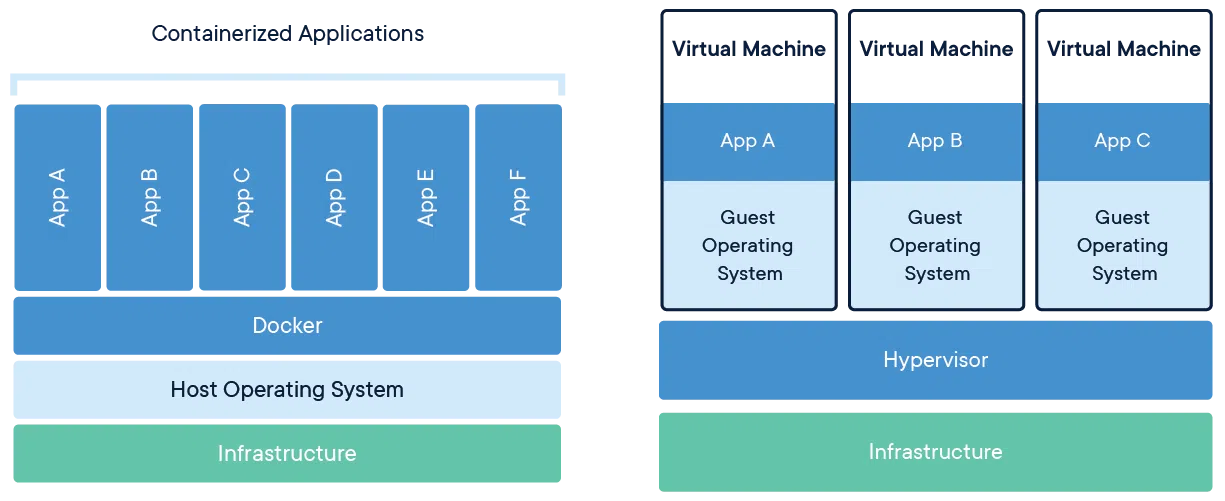
\includegraphics[width=0.75\linewidth]{figures/docker-containerized-and-vm-transparent-bg.png.jpg}
	\centering
	\caption{Comparing Containers and Virtual Machines. \href{https://www.docker.com/resources/what-container/}{[Ref]}}
	\label{ComparingContainersandVirtualMachines}
\end{figure}

\subsection{Docker network}

Containers, as they are referred to, represent these isolated environments. They are interconnected through the advanced Docker network~\cite{DockerNetwork}, which offers a wide array of options and configurations, ensuring high availability for any given setup. This isolation, while also allowing communication between the containers when needed , facilitates the creation of highly scalable and secure applications for future upgrades and optimizations. In contrast to traditional virtualization, Docker images and their associated containers can be incorporated into other applications with minimal configurations, making the project easier to deploy and even adjust in environments that are already deployed.

\subsection{Docker compose}

Docker Compose~\cite{DockerCompose} is a tool that enables the operation of multi-container Docker applications. It serves as the connecting link, providing a simple and organized interface for running multiple containers in conjunction with each other. It offers an ideal environment for both development and smaller scale production applications, allowing developers to have an organized view of their application's configuration, networking and simplifying the development process. Through its interface, developers can coordinate both official and custom images, integrating them into their application as needed. Docker Compose aligns with the DevOps principles, aiming to bridge the gap between the development and the actual functionality of an application.

Today's leading cloud service providers offer near-native support for containerized applications, making Docker tools an excellent choice for managing the development process. This support significantly simplifies the transition from simple IoT implementations to production-level deployments on a cloud provider, making the experience more seamless and intuitive.

\section{Event Streaming}\label{event_streaming}

Event streaming is the process of capturing real time data from a variety of event sources like sensors, devices, gateways, databases and other cloud services. Apache Kafka \cite{WhatIsApacheKafka} is a relatively recent technology that introduces the concept of event streaming to the cloud community. The main flow scheme utilized here is publish/produce, store, subscribe/consume. This model is versatile and can be applied to nearly any type of cloud communication , its primary function being to handle large amount messages per second.

\subsection{Apache Kafka}

Apache Kafka provides low latency, high throughput, scalability and high availability. Kafka enables the use of high-volume real-time data transfer with low latency and provides temporary storage for short-term usage. In contrast, the conventional database model requires all produced data to be first stored in the database before it can be used for any given task. Kafka can be viewed as a cloud cache, offering high availability and low latency , which makes it an excellent choice for real-time event streaming applications. Event streaming is leveraged across a wide spectrum of use cases, including activity tracking for real-time insights, processing data in real-time for immediate decision making, providing low latency and fault-tolerant messaging for critical systems , monitoring operational data to maintain system health and aggregating logs for efficient analysis and troubleshooting.

\subsection{Events}
\label{events}
Events or event records are the messages that contain the information about an actual event that happened (in a structured manner) and they are the main way of reading and writing data to Kafka. An event mainly consists of a key, a value and a timestamp.
Each event within the same topic is distinguished by a unique key. The key determines how these events are distributed across different partitions (cf. Sec. \hyperref[kafka_topics]{3.2.4} \hyperref[kafka_partitions]{ 3.2.5}).
The value is the actual data that is distributed and varies from simple text, to JSON file and even more complex formats like Avro \cite{Avro}, that are encoded properly and stored in the Kafka topics. The timestamp contains information about the time that each event took place.

In the following example, the key 'MqttSensor1' uniquely identifies the source of the data produced or consumed by a Kafka topic. The value 'Mqtt sensor 1 measured $25^{\circ}C$' represents the actual data recorded and the timestamp 'Jul. 15, 2022 at 12:56 a.m.' indicates when this measurement was taken.
\begin{itemize}
    \item Key: 'sensor1'
    \item Value: 'Sensor 1 measured 22.5 \si{\celsius}'
    \item Timestamp: '2/3/2024, 3:14:23 PM'
    % \item Optional metadata
\end{itemize}

\subsection{Brokers}
Brokers serve as the primary infrastructure where data is temporarily stored for subsequent processing, before being pushed for long-term storage. Brokers are organized into clusters, allowing for multi-broker and multi-cluster setups. We do not delve into multi-cluster implementations, since they are primarily used in large-scale multi-region enterprise applications \cite{MultiClusterImplementation}. The complexity and operational overhead of managing multiple clusters is not justifiable for most IoT applications, since our single-cluster implementation meets the requirements for high throughput, fault-tolerance and low latency. 

In the past, Kafka was utilizing Zookeeper \cite{zookeeper} to orchestrate the communication between the Kafka broker nodes and the metadata management. But now, a new protocol called KRaft(Kafka Raft metadata mode) \cite{Kraft} has been implemented to act as the new quorum controller and has a more direct connection to all the Kafka nodes. Nodes can function as a controller, a broker, or both, as depicted in Figure \ref{Kafka_Internals_052}. Controller nodes , deployed as Kafka images, play a crucial role in storing all the necessary metadata for managing the distribution and synchronization of data across the broker nodes.

\begin{figure}[htbp]
	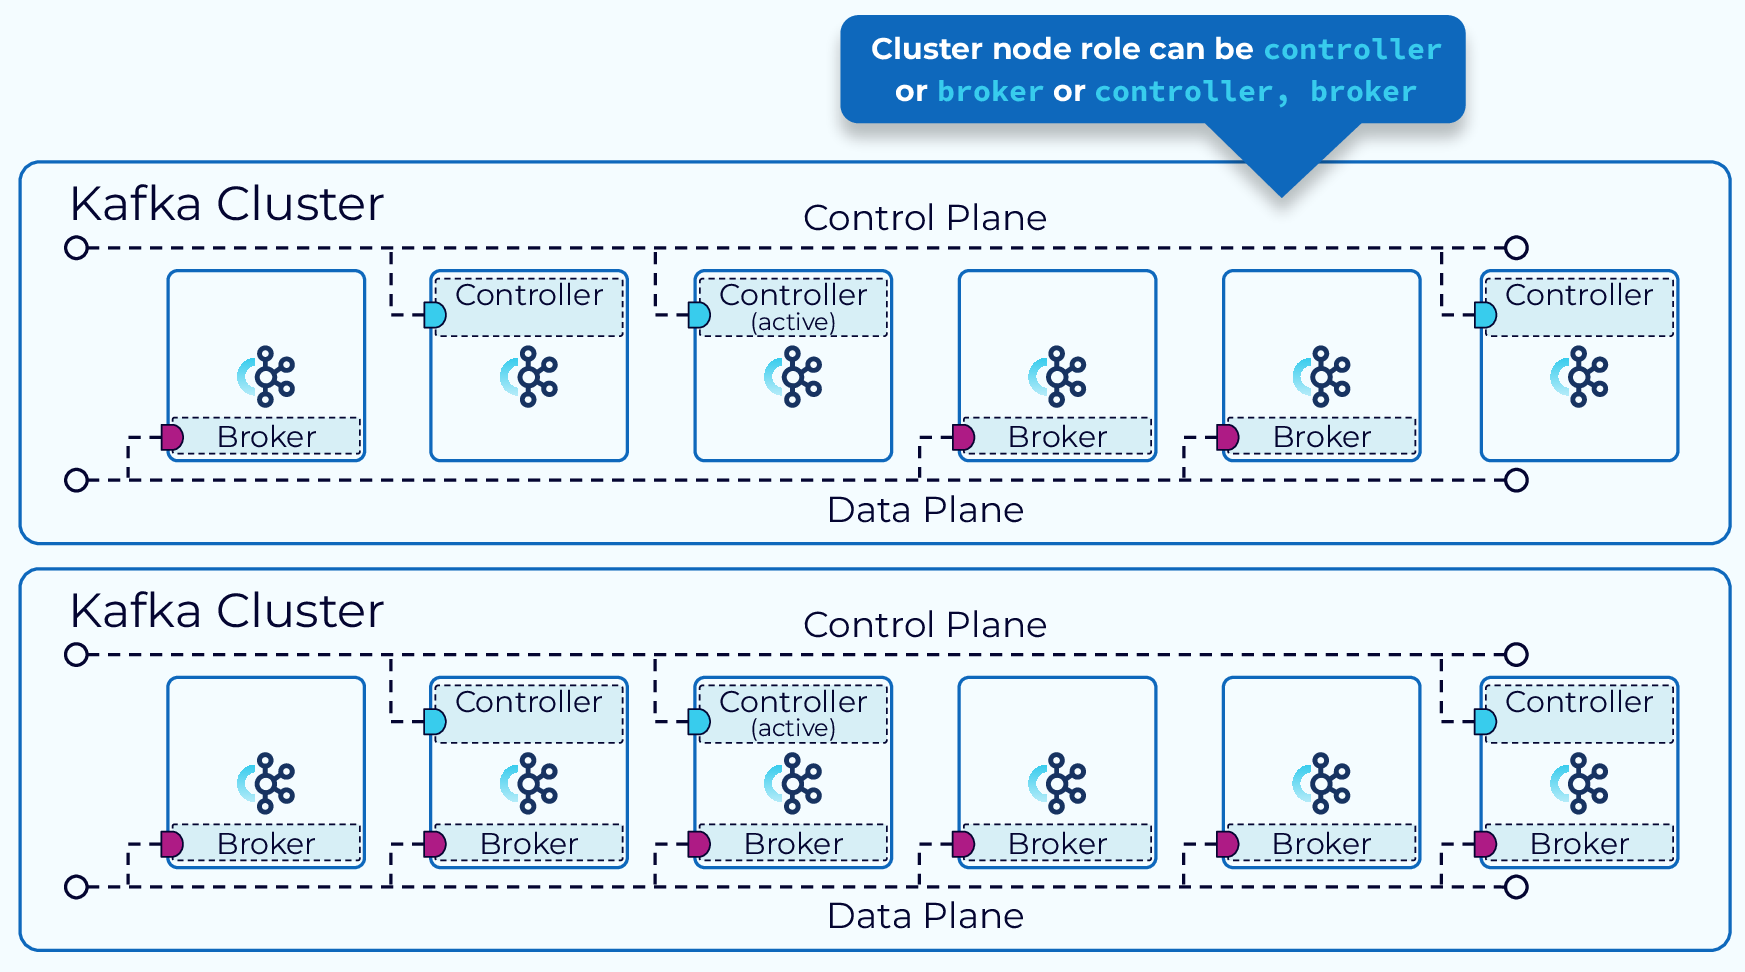
\includegraphics[width=0.75\linewidth]{figures/Kafka_Internals_052.png}
	\centering
	\caption{KRaft Cluster Node Roles. \href{https://developer.confluent.io/courses/architecture/control-plane/}{[Ref]}}
	\label{Kafka_Internals_052}
\end{figure}

Applying the correct configurations, each Kafka cluster in a multi-broker implementation becomes fault tolerant. Kafka controllers are responsible for the load balancing and the fault tolerance of any Kafka application. 
Furthermore, Kafka's ability to provide high throughput and low latency ensures that applications using it are not only fast and responsive, but also safeguarded against data losses due to run time failures. Multi broker implementations combined with the new KRaft control protocol offer faster response times whenever data recovery is needed, which usually occurs in the case that one or more brokers fail during their operation. In alignment with the Apache Kafka project's current recommendation, we have opted to use KRaft as the controller in our thesis, replacing Zookeeper, which has been deprecated for new deployments \cite{KraftRecommendation}.

\subsection{Kafka Topics}\label{kafka_topics}
Going a step further, Kafka uses topics to manage and securely store events. Topics function like folders in a file system, with events acting as the files within. New event messages are appended to the end of the topic and, once written, these events are unchangeable. In Kafka topics, unlike other messaging systems, events are not deleted post-consumption. Instead, a retention period is set, beyond which messages are deleted, with the maximum duration being up to one week. The performance of Kafka remains stable regardless of data stored, implying that long-term data storage should have a minimal performance impact.
\subsection{Kafka Partitions}\label{kafka_partitions}

\begin{figure}[htbp]
	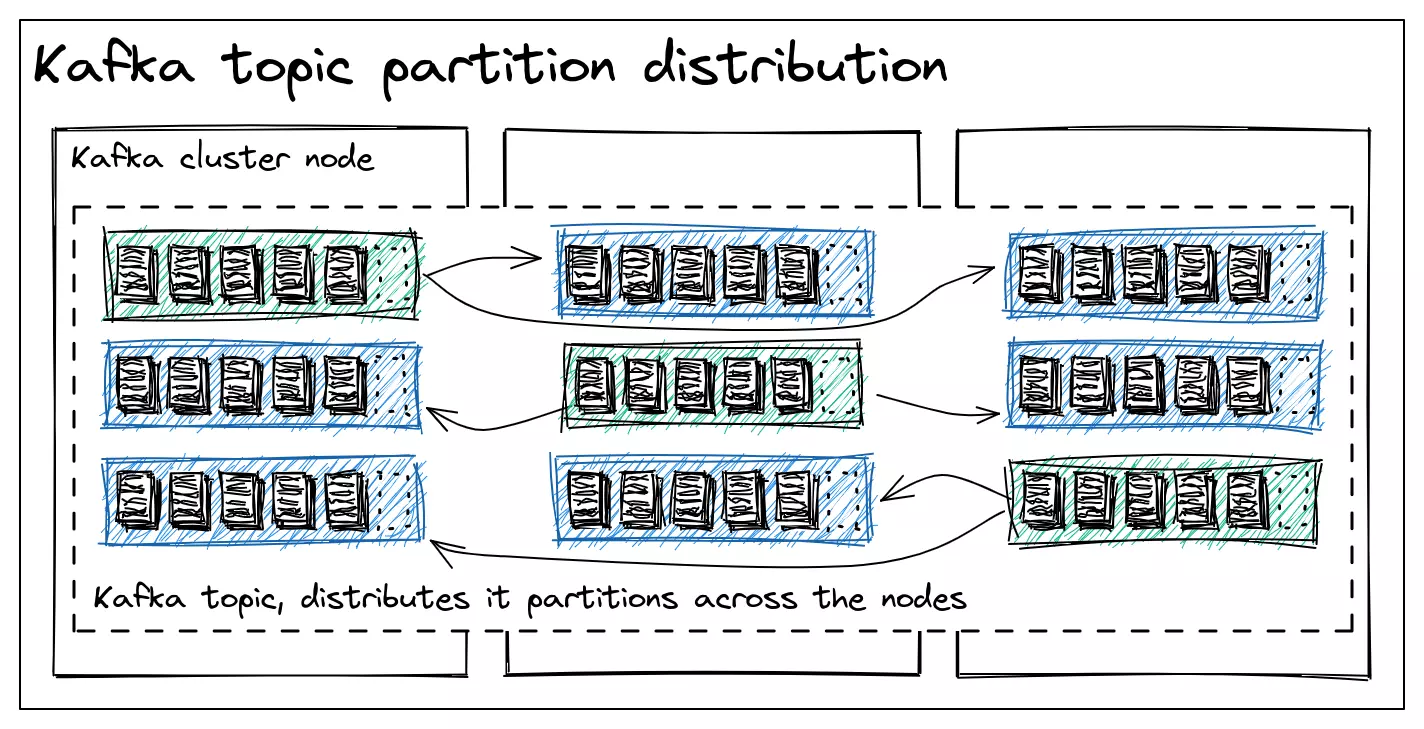
\includegraphics[width=0.75\linewidth]{figures/partition-distribution.jpg}
	\centering
	\caption{Kafka topic partition distribution. \href{https://trigodev.com/de-at/blog/kafka-topics-and-partitions}{[Ref]}}
	\label{PartitionDistribution}
\end{figure}

Kafka topics are segmented into partitions. A single topic in Kafka is divided into multiple partitions . Partitions are distributed across Kafka brokers in the cluster and messages are shared among multiple nodes. The performance of reading, writing and processing events is maximized and data is replicated across all Kafka nodes, presented in Figure \ref{PartitionDistribution}. New events are appended to a specific partition within a topic and events with the same key are stored in the same partition, ensuring data ordering. This partitioning mechanism contributes to the high throughput and fault tolerance capabilities of Kafka.

\section{Existing Event Streaming Protocol Integration}
We support different protocols currently available on the SYNAISTHISI platform. Since most IoT devices and applications primarily use the RabbitMQ and MQTT protocols, our primary focus is to interconnect these protocols with our Kafka components.
\subsection{RabbitMQ}
RabbitMQ \cite{RabbitMQ} is an open-source message broker, also known as a message-oriented middle-ware. It implements the Advanced Message Queuing Protocol (AMQP) and supports several other protocols. RabbitMQ provides robust messaging for applications. It is easy to use, runs on all major operating systems and supports a huge number of developer platforms. It also provides a wide range of features to let you trade off performance with reliability, in means of persistence, delivery acknowledgments and high availability. The key supported protocols are AMQP, MQTT, STOPMP, HTTP and Web Sockets. Additionally, it offers multi-language client support, providing a wide range of development platforms of the most popular programming languages and frameworks like Python, Java, .NET, JavaScript, Ruby, Go, etc. RabbitMQ can be deployed in distributed and federated configurations to meet high scale and availability requirements. It offers flexible routing and bridging mechanisms, along with fault tolerance features such as clustering, automatic fail-over and message durability. This wide variety of protocol support and accessible bridging between those protocols make RabbitMQ a valuable tool for the IoT market, while worldwide large-scale companies also use it, mainly for their messaging infrastructure.
\subsection{MQTT}
MQTT \cite{MQTT} stands for Message Queuing Telemetry Transport. It is a lightweight publish-subscribe network protocol capable of transporting messages. It is designed for restricted devices and low-bandwidth, high-latency, or unreliable networks. The protocol ensures reliable message delivery and minimizes network bandwidth requirements. It provides one-to-many message distribution applications and message retainment, since an MQTT topic holds the last messages and the next time a client subscribes, it immediately receives these messages. The low transport overhead and quality of service options provided by MQTT make it an ideal choice for scenarios where network bandwidth is limited and connectivity is unreliable. Thus, its lightweight nature and efficient use of network resources make MQTT a popular choice in the IoT ecosystem, where devices often operate under unstable network conditions and power limitations.

\section{Kafka Connect}
\label{kafka_connect}
Kafka Connect \cite{KafkaConnect} is a robust framework that allow us to interconnect our Kafka cluster with external systems such as databases, search indexes and different kinds of communication protocols. It is designed to handle various event streaming use-cases, including scalable and reliable streaming of data to and from Kafka. The framework is designed around a simple concept of connectors and workers. Source connectors import data from systems and propagate it to Kafka, while Sink connectors export data from Kafka to external systems. Connectors manage the integration between Kafka and other systems and they can be created without the necessity of additional code to be written. Each time we add a new external framework to our stack , we usually need to write the code that interconnects it with our Kafka cluster. Ηowever, this type of code does not provide any advantage to our application compared to other similar applications, especially in systems where a lot of services that need to communicate with each other are involved. This resolves much trouble during the development time of a specific application, as it removes the necessity of writing undifferentiated code for those external interfaces every time a new one is incorporated. All undifferentiated code interfacing with other systems is bundled into separate libraries, allowing us to deploy only the necessary connectors. Furthermore, Kafka Connect is a highly acceptable solution for interconnecting different protocols to our Kafka implementation. 

Connect uses numerous connectors, among which we utilize the RabbitMQ and MQTT source-sink connectors. This allows us to interconnect these protocols that already exist in the SYNAISTHISI platform with Kafka. If necessary, we could indeed create our own connectors, providing us with the flexibility to manage virtually any data integration requirement. Kafka Connect includes a REST API for managing and monitoring connectors through workers. This API allows us to deploy, remove, pause, resume and check the status of workers associated with their corresponding connector. Automatic offset management is provided, therefore in case a connector fails, the replacement can resume exactly where the previous one stopped, guaranteeing data consistency. Kafka Connect is a powerful tool that simplifies the process of integrating different systems with Kafka and empowers robust, scalable and reliable data pipelines in our implementation. 

\section{Schema Registry}
Kafka Schema Registry \cite{SchemaRegistry} offers a REST interface for storing and retrieving schema registries and is an essential part of the Apache Kafka ecosystem. Its role is crucial in maintaining the consistency and well-defined nature of the data in Kafka topics. Kafka Schema Registry is used in combination with Apache Avro \cite{Avro}, providing a data serialization system that encodes data in a compact binary format . Avro schemas define the structure of the data being encoded, making it easy for each consumer to correctly deserialize the data. This advanced and compact binary format allows us to significantly reduce the event’s message size, especially in instances where the producer is utilizing the JSON format.


\begin{figure}[htbp]
	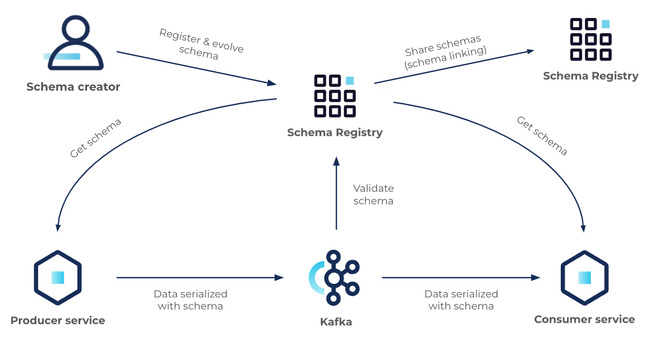
\includegraphics[width=0.75\linewidth]{figures/schema-registry-ecosystem.jpg}
	\centering
	\caption{Schema Registry architecture overview \href{https://docs.confluent.io/platform/current/schema-registry/index.html}{[Ref]}}
	\label{SchemaRegistryEcosystem}
\end{figure}

The primary purpose of a schema registry, is storing and retrieving schemas in a centralized location, presented in Figure \ref{SchemaRegistryEcosystem}. Producers and consumers that utilize schema registry, own a contract of what type of data to expect, reducing the possibility of data inconsistency and parsing errors . Schema evolution is supported to accommodate the inevitable changes in our data over time, reflecting the evolving needs of our applications. This ensures our system remains flexible and adaptable to meet these ongoing changes. The support for schema versioning in our system allows us to maintain compatibility with older data that was encoded using previous versions of the schema, providing seamless access and utilization of older data structures. 

In summary, Schema Registry is a crucial tool for maintaining compatibility and data integrity in Kafka-based systems. It provides a centralized store for schemas, supports schema versioning and evolution and allows for a clear contract between producers and consumers. Over the past few years, it has emerged as an industry standard for event streaming applications, driven by the increasing need for data size reduction and compatibility in the face of growing data volumes and complex processing requirements.